\documentclass[12pt]{article}

\usepackage{graphicx}
\graphicspath{{./img/}}

\pagenumbering{arabic}

% VARIABLES
\def\UART_VERSION{v1.0.0}

\begin{document}
\begin{titlepage}
  \centering
  {\LARGE \textsc{Uart Implementation Reference}\par}
  {\vspace{1cm}}
  \UART_VERSION \\
  {\vspace{16cm}}
  Written by \\
  Kevin LASTRA
\end{titlepage}
\tableofcontents
\newpage

\section{Introduction}

\subsection{Purpose of the manual}
The purpose of this manual is twofold. First, it serves as a 
comprehensive resource to document the Implementation of a 
Universal Asynchronous Receiver-Transmitter (UART). This process 
has been undertaken not only as a journey of self-learning but also 
as a way to share knowledge and contribute to the broader community
of developers, engineers, and enthusiasts.

\subsection{Audience}
This manual is primarly intended for design engineers who are 
involved in the development and implementation of communication
systems, particularly those working with embedded systems, 
microcontrollers, and hardware interfaces.

\newpage
\section{UART overview}
The Universal Asynchronous Receiver-Transmitter (UART) is a 
fundamental hardware communication protocol used for asynchronous
serial communication. \\
This protocol is widely used in embedded systems, 
microcontrollers, and communication devices due to its simplicity and effectiveness
in handling relatively low-speed data transfer.
\subsection{UART fundamentals}
\subsubsection{Reception and transmission}
UART allows two devices to exchange data using only two wires, RX for receive data
and TX for transmit data.\\
\begin{figure}[h]
  \centering
  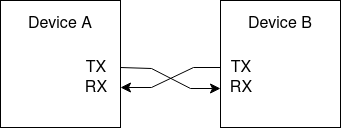
\includegraphics[scale=0.6]{UART_interface.drawio.png}
  \caption{Two UART's interfaces connected}
\end{figure}


\subsubsection{Asynchronous communication}
An asynchronous communication refers to a type of data transmission where the sender
and receiver do not rely on a shared clock signal for synchronization. Instead, each
device operates using its own internal clock and relies on specific timing 
conventions to ensure data is transmitted and received correctly. \\~\\
In asynchronous UART communication, the data is sent in discrete chunks 
(called data frames) over the communication channel, with the timing governed by 
agreed-upon parameters like baud rate and frame size.

\subsubsection{Baud rate}
The baud rate defines the speed at which data is transmitted over the communication
channel. It is usually expressed in bits per second (bps). \\
In the context of UART the baud rate specifies how many bits of data can be 
transmitted each second. Both transmitter and receiver must be set to the same baud
rate. \\~\\
The general formula for calculating the baud rate is:

\[Baud Rate = \frac{Clock Frequency}{Divisor}\]

\subsubsection{Data frame structure}
A UART data frame typically consists of: \\

\begin{tabular}{|p{3cm}|p{6cm}|p{3.5cm}|}
  \hline
  \textbf{Range name} & \textbf{Description} & \textbf{Implementation bit length} \\
  \hline
  Start bit & Signals the beginning of data transmission & 1 \\
  \hline
  Data bits & The actual data being sent & 5 - 9 \\
  \hline
  Parity & Used for error checking & 0 - 1 \\
  \hline
  Stop bit & Signals the end of the data transmission & 1 - 2 \\
  \hline
\end{tabular}

\subsection{Advantages and limitations}
Advantages:
\begin{enumerate}
  \item Minimal pins required, essay to implement on a system.
  \item Low cost, because of its minimal hardware requirements the UART is a
        cost-effective solution.
  \item Widely supported.
  \item Simplicity in software implementation.
\end{enumerate}
limitations:
\begin{enumerate}
  \item Distance limitations, the maximum range depends on the baud rate, the quality
        of the wires and the environment (e.g. electromagnetic interferences).
  \item Relatively slow data transfer.
  \item Limited to two devices.
  \item Susceptibility to baud rate mismatch.
  \item Limited error detection, UART error detection is limited to parity checks and
        stop bits.
\end{enumerate}

\section{Implementation}

\subsection{Design}
\subsection{Interface}
\subsection{Registers}
\subsection{Interrupt request (IRQ)}
\subsection{Low power}
\end{document}